%%%%%%%%%%%%%%%%%%%%%%%%%%%%%%%%%%%%%%%%%%%%%%%%%%%%%%%%%%%%%%%%%%%%%%%
%%%%  Load the document class and packages                         %%%%
%%%%%%%%%%%%%%%%%%%%%%%%%%%%%%%%%%%%%%%%%%%%%%%%%%%%%%%%%%%%%%%%%%%%%%%
\documentclass[a4paper]{report}
\usepackage{epsfig}            % to insert PostScript figures
\graphicspath{ 
  {figures/} 
}

%Change figure names
\renewcommand{\figurename}{Fig}

\usepackage[bf,footnotesize]{caption} % make captions small and label bold


\addtocounter{chapter}{1} %Because starting at zero is silly
\makeatletter
\renewcommand{\thesection}{\@arabic\c@section}
\renewcommand{\thefigure}{\@arabic\c@figure}
\makeatother

\usepackage[a4paper,margin=2.7cm,tmargin=2.5cm,bmargin=2.5cm]{geometry} 
\usepackage{textcomp}          % To make nice degree symbols and others\usepackage[bf,footnotesize]{caption} % make captions small and label bold
\usepackage{wrapfig}
%to produce the clickable references along the left in Acroread. This
%package must be included last. 
\usepackage[ps2pdf,bookmarks=TRUE]{hyperref} 



%%%%%%%%%%%%%%%%%%%%%%%%%%%%%%%%%%%%%%%%%%%%%%%%%%%%%%%%%%%%%%%%%%%%%%%
%%%%  Hypertext references for Acrobat                             %%%%
%%%%%%%%%%%%%%%%%%%%%%%%%%%%%%%%%%%%%%%%%%%%%%%%%%%%%%%%%%%%%%%%%%%%%%%
\hypersetup{
pdfauthor = {TENSS},
pdftitle = {Laser Alignment},
pdfkeywords = {lasers,optics,alignment,reflection,microscopy},
pdfcreator = {LaTeX with hyperref},
pdfproducer = {dvips + ps2pdf}
           }


\begin{document}




%set the number of sectioning levels 
\setcounter{secnumdepth}{2}

\begin{center}
\textbf{\Large{Laser Routing and Alignment}}
\end{center}

A thorough understanding of beam alignment is absolutely critical for being able to build a scanning microscope. 
When we say `beam alignment' we refer to the process of routing a laser beam precisely along a defined path. 
This is achieved using small, flat, \textit{first surface} mirrors mounted on holders with fine adjustment jobs.
Optical elements such as lenses are generally inserted into the path defined by the beam. 



\section{Aligning the beam through a path defined by two points}
The aim of this exercise is to use mirrors to redirect a laser beam coming in at an arbitrary angle through a specific line at a specific height above the table.
Do not touch the mirror surfaces! 
They are delicate.
You will set up a laser pointer, two mirrors, and two irises in order to achieve the state shown in Fig.~\ref{fig:ex1}. 
The irises and $mirror_2$ are shown mounted on a rail, but this isn't necessary. 
You can also clamp these three components to the breadboard.
The only restriction is that they need to form a line. 
Separate the irises by as much space as possible and keep $mirror_2$ fairly close to $iris_1$.
Once this is established, add $mirror_1$ such that it is square with $mirror_2$ and at least about $10~cm$ away from it. 
Finally, set up the laser pointer such that the beam hits $mirror_1$.
Now the fun starts\ldots


\begin{figure}[h]
\center
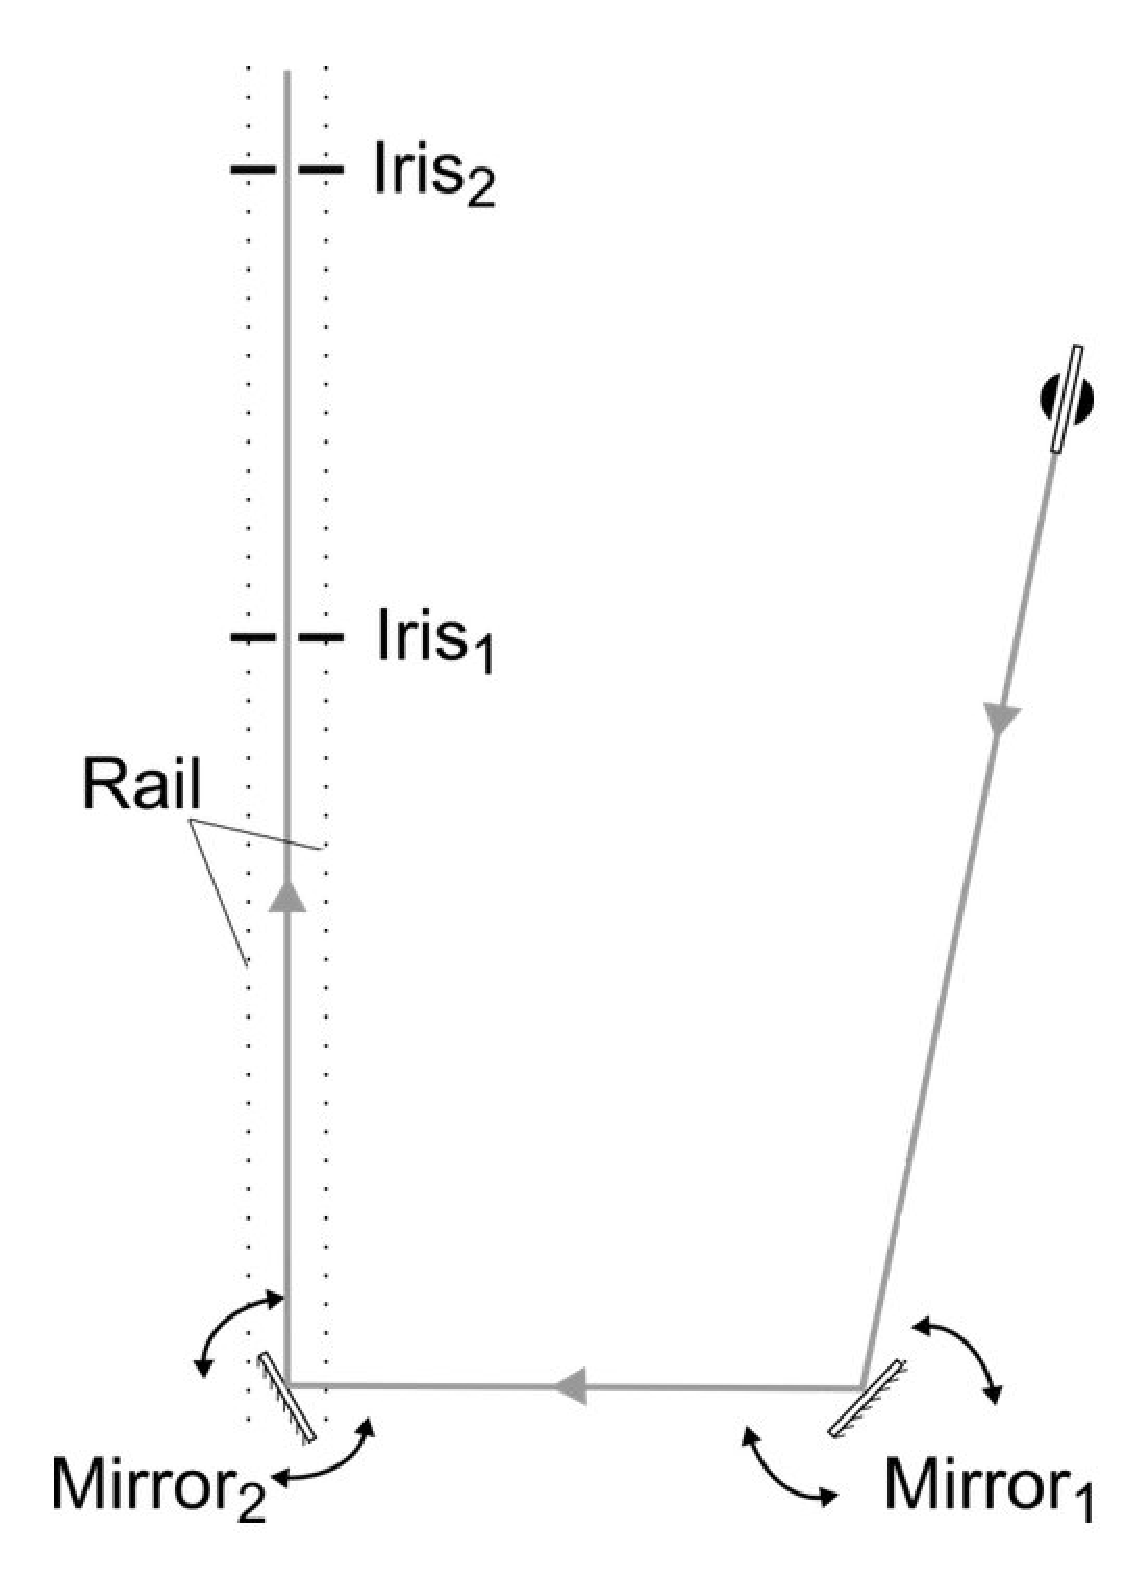
\includegraphics[width=2.25in]{laser_alignment_exercise_basic.eps}
\caption{Your goal is to send the beam through the two irises by altering the tilt of the two mirrors.}
\label{fig:ex1}
\end{figure}


The goal is to have the beam pass through the two iris centres without moving the laser pointer. 
In most cases it will be possible to complete the exercise simply by altering the tilt of the mirrors and rotating the mirror posts in their holders. 
If the mirrors are initially very mis-positioned you might also need to translate them across the table. 
To complete the exercise you will need to understand the following keys points:

\begin{enumerate}
\item Adjusting $mirror_1$ \textit{translates} the beam across the surface of $mirror_2$.
\item Adjusting $mirror_2$ alters \textit{the angle} with which the beam goes through the irises. 
\item As a consequence of (1), you adjust $mirror_1$ to pass the beam through $iris_1$.
\item As a consequence of (2), you adjust $mirror_2$ to pass the beam through $iris_2$.
\item Iteratively adjusting the two mirrors will always allow the beam to pass through both irises, \textit{assuming there exists a region of $mirror_2$ that falls along the axis defined by the two irises.} 
\end{enumerate}

\clearpage
Here is how you will implement the above:

\begin{enumerate}
\item Close $iris_1$ and adjust $mirror_1$ to position the beam at the centre of $iris_1$.
\item Open $iris_1$ and rotate $mirror_2$ to position beam at centre of closed $iris_2$. 
The process of doing this will move the beam away from the centre of $iris_1$. 
The degree to which this happens depends on the distance between $mirror_2$ and $iris_1$.
\item Close $iris_1$ and assess the beam position. If not aligned, repeat steps 1 \& 2. 
If aligned, stop. 
\end{enumerate}

\subsubsection{Tips}
\begin{itemize}
\item If after repeated attempts at alignment you keep failing, this indicates that a mirror (probably $mirror_2$) is mis-positioned. 
\item Keep everything roughly at right angles. 
      Whilst it is possible to use very acute angles and still solve the alignment task, you will have a larger mirror area to play with if you reflect the beam at 90 degree angles.
\item Manage your real-estate: You will notice that sometimes, the beam will fall off $mirror_2$. 
      This problem can be solved by translating $mirror_2$ in the direction where the beam fell off its edge.
\end{itemize}


\section{Getting the beam parallel with the table}
Your large 2-photon laser has arrived and it's time to begin building your microscope's light path. 
To make your life easier, you decide to use two mirrors to ensure the beam emerging from the laser is parallel with the optical table and at a height suitable for your lenses and other optical elements. 
Set up your laser pointer and two mirrors as shown in Fig.~\ref{fig:ex2}. 
The mirrors can be as close to the laser as you like. 
Place an iris on a post holder and use a post base to improve stability. 
Do not bolt the iris to the table.
This single iris defines the height at which you want the beam to be at all locations on the optical table. 
Based on what you learned in Exercise 1, use the iris and the two mirrors to ensure the beam is parallel with the table at the height defined by your iris. 
Hint: all you're allowed to do is change the tilt of the two mirrors and move iris.


\begin{figure}[h]
\center
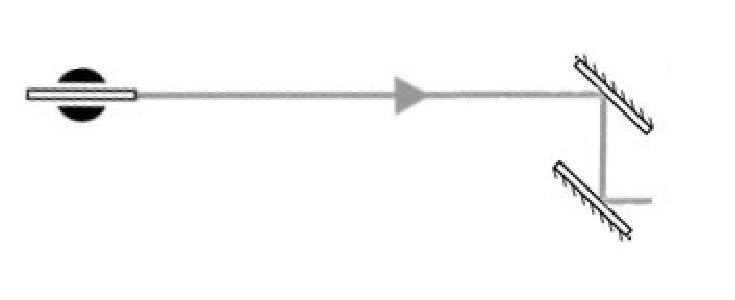
\includegraphics[width=4in]{laser_height.eps}
\caption{Using two mirrors to ensure the beam is parallel with the table. }
\label{fig:ex2}
\end{figure}



\end{document}
